\setcounter{figure}{0}
\setcounter{table}{0}
\setcounter{equation}{0}
\section{Matlab程序设计和GUI设计}
Matlab是一个功能极其强大的数据处理软件,传统的数据分析和处理都是人工计算,在面对一些复杂的计算时,会耗费大量的时间和精力,这就使效率低下。利用计算机进行数据处理,可以将一些重复的、复杂的计算快速准确地进行。利用计算机处理数据,除了可以省时省力外,可以将做过一次数据处理的源码保存下来,下一次进行同类型数据处理的时候可以重复利用。Matlab不仅仅可以进行数据处理,它还支持人机交互界面的设计,也就是Matlab的图形用户界面GUI。这就使得数据处理变的直观,非专业人士也可以轻松地使用别人开发好的GUI数据处理程序来完成一些数据的分析与处理。
\subsection{Matlab基本操作}
\subsubsection{Matlab的数据基础}
在Matlab中,用数组和cell来存储任何数据,所有的数据处理是基于变量的操作。
\begin{enumerate}
	\item \textbf{数组}
	\begin{enumerate}
		\item 一维数组
		
		\qquad 数组就是数据的有序集合,一维数组可以看成向量,在处理的时候可以对一组有联系的数据以数组的形式赋值给变量。常用创建数组和获取数组数据的形式如下:
		\begin{lstlisting}
 >> a = [1 2 3 4 5];			% 直接输入创建一维数组,元素可以用空格或逗号隔开
    a = 
		1	2	3	4	5
 >> b = 1:2:9;					% 利用start:step:end 形式创建一维数组
	b =
		1	3	5	7	9
 >> a(3)						% 用变量名加下标的形式获取数组元素
 	ans = 
 		3\end{lstlisting}
		\item 二维数组
		
		\qquad 二维数组可以作为矩阵,常用的创建和获取数组数据方法如下:
		\begin{lstlisting}
 >> a = [1 2 3;4 5 6;7 8 9]		% 直接输入创建二维数组,用“ ; ”换行
    a = 
    	1	2	3
    	4	5	6
    	7	8	9
 >> b = [1 2 3					% 直接输入创建二维数组,手动换行
 		 4 5 6
 		 7 8 9]
	b = 
	 	1	2	3
	 	4	5	6
	 	7	8	9
 >> a(2,2)						% 用变量名加下标来获取元素,二维数组用行数和列数来确定元素
 	ans = 
 		5\end{lstlisting}
	\end{enumerate}
	\item \textbf{cell}
	
	\qquad cell数组也是数组,它也可以是一维和二维,它的特殊之处就是它可以存放任何数据,也就是说它的元素可以是字符串,单个数据,甚至是数组。cell数组的使用方法如下:
	\begin{lstlisting}
 >> a = [1 2 3 4 5];				% 创建一维数组
 >> b = [1 2 3;4 5 6;7 8 9];		% 创建二维数组
 >> c = 'hello';					% 创建字符串
 >> d = {a,b,c}						% 赋值给 cell 数组
 	d = 
 		[1x5 double]	[3x3 double]	'Hello'
 >> d(1)							% 获取元素用“ ( ) ”,不能获取内容
 	ans =
 		[1x5 double]
 >> d{1}							% 获取元素内容用“ { } ”
 	ans =
 		1	2	3	4	5\end{lstlisting}
\end{enumerate}
\subsubsection{Matlab常用函数}
Matlab计算功能之所以强大,是因为它拥有很多的工具箱,里面封装了许多用于处理数据的函数,掌握如何使用这些函数,就掌握了Matlab的使用。在误差理论与数据处理中,常用的Matlab函数如表2-1:
\begin{figure}[H]
	\centering
	\captionsetup{type=table}
	\caption{\textbf{Matlab常用误差处理函数}}
	\begin{tabular}{p{3cm}<{\centering}p{8cm}}
		\toprule
		\textbf{函数}&\multicolumn{1}{c}{\textbf{作用}}	\\
		\midrule
		length(a)	&获取一维数组的长度\\
		size(A)	&获取二维数组的行与列\\
		max(A)	&获取数组A的最大值\\
		min(A)	&获取数组A的最小值\\
		mean(A)	&获取数组A的平均值\\
		sqrt(n)	&获取数值n的算术平方根\\
		std(X)	&获取数据X的标准差\\
		inv(A)	&获取矩阵的逆矩阵\\
		floor(x)	&获取小于x的最大整数\\
		ceil(x)	&获取大于x的最小整数\\
		roundn(x,n)	&对x进行四舍五入,数据精度为$ 10^n $\\
		\bottomrule
	\end{tabular}
\end{figure}
\subsubsection{Matlab绘制图像}
无论是处理数据和误差分析,还是进行别的数学计算处理的时候,绘制函数图形能更直接地了解数据的特性,也可以更直接地描述出计算的结果。在Matlab中,绘制函数图形的功能也是很强大的。在Matlab中常用绘图方法:
\begin{lstlisting}
 >> x = 0:0.01:2*pi;					% 产生一组数据 x
 >> y = sin(x);							% 用 sin 函数产生 y
 >> plot(x,y,'-b')						% 绘制函数图像,‘ - ’设置线条类型,‘ b ’设置颜色
 >> grid on								% 设置显示网格
 >> title('the function of sin')		% 设置图像标题
 >> xlabel('x')							% 设置 x 坐标名称
 >> ylabel('y')							% 设置 y 坐标名称\end{lstlisting}
 绘制的结果如下图:
\begin{figure}[H]
	\centering
	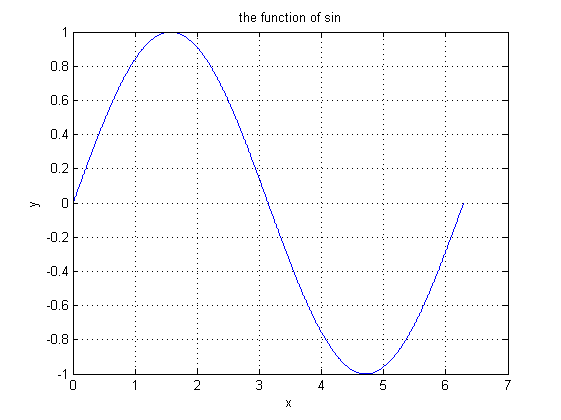
\includegraphics[scale=0.6]{sin_x}
	\caption{\textbf{$ sin(x) $的函数图像}}
\end{figure}
\subsubsection{Matlab的m文件}
Matlab编写的代码是以.m结尾的文件格式,m文件分为两种,m脚本文件和m函数文件。将执行的命令集写在m脚本文件中,直接在命令窗口输入文件名即可运行脚本文件,为了使文件不与Matlab自带的命令冲突,不要把文件命名与Matlab自带命令名称一致。编写脚本如下:
\begin{lstlisting}
   x = 0:0.01:2*pi;
   y = sin(x);
   plot(x,y,'-b')
   grid on
   title('the function of sin')
   xlabel('x')
   ylabel('y')\end{lstlisting}
将上面代码保存为plotsin.m文件,在命令窗口输入plotsin也可以绘制出图2-1函数图像。

还有一种是m函数文件,它在文件内部定义一个函数,由外界调取该函数进行计算,不可以单独运行,定义的函数名称要与文件名称一致,且不能与Matlab自带函数名称冲突。编写代码如下:
\begin{lstlisting}
 function sum = adds(x, y)
 sum = x + y;\end{lstlisting}
将上面代码保存为adds.m文件,在命令窗口输入adds(3,4),执行结果如下:
\begin{lstlisting}
 >> adds(3,4)
 	ans =
		 7\end{lstlisting}
\subsection{Matlab GUI设计}
在Matlab中,GUI设计有两种方法,一种是用代码实现界面的编程,还有一种是使用GUIDE图形界面设计,前者虽然编写代码量较大,界面的绘制都用代码实现,但在重复设计上有优势,比如大部分控件拥有相同的属性,在这里可以用循环来设置。后者虽然操作简单,界面绘制布局可视化,但在控件多的情况下,重复设置属性就比较麻烦了。在本毕业设计中,采用的前种设计方法。在Matlab中图形界面的层次结构如图2-2\scite{4}。
\begin{figure}[H]
	\centering
	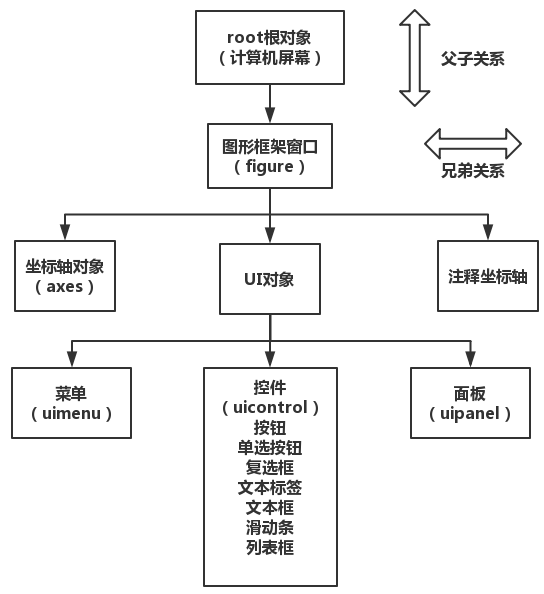
\includegraphics[scale=0.5]{MatlabGUI}
	\caption{\textbf{GUI对象层次结构图}}
\end{figure}
\subsubsection{Matlab中设计GUI的函数}
\begin{enumerate}
	\item \textbf{figure函数\scite{4}}

	\qquad 根据图2-2的结构图,设计图形界面首先要设计一个图形框架窗口,设计的方法如下:
	\begin{lstlisting}
 hf = figure('PropertyName',propertyvalue,...);\end{lstlisting}
 	其中:hf为对象名,函数的参数是成对存在的属性PropertyName和属性值propertyvalue,用来设置图形框架窗口的一些属性。比如执行如下代码:
	\begin{lstlisting}
 hf = figure('Name','MyFigure',...					% 设置窗口名称
    'NumberTitle','off',...							% 设置是否显示窗口编号
    'Position',[200,200,600,450],...				% 设置窗口的位置和大小
    'MenuBar','none',...							% 设置是否显示自带菜单
    'Color','White',...								% 设置界面颜色
    'Resize','off');								% 设置界面大小是否可变\end{lstlisting}
	上面代码可以在命令窗口和m文件内执行,执行结果如图2-3:
	\begin{figure}[H]
		\centering
		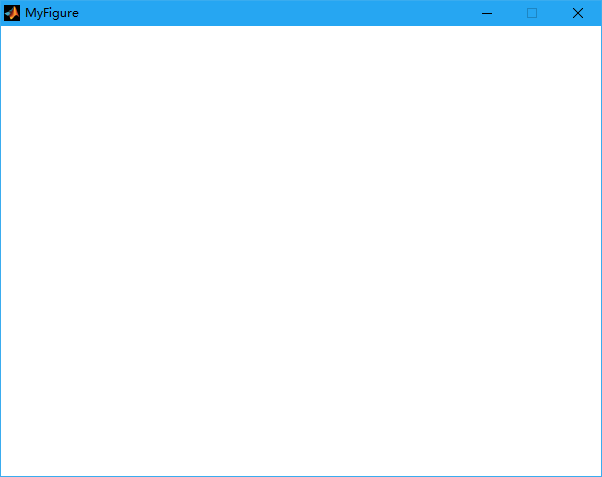
\includegraphics[scale=0.4]{MyFigure}
		\caption{\textbf{MyFigure窗口}}
	\end{figure}
	根据图2-3的结果,窗口的位置和大小都是固定的,而且窗口是不可变的,不能拖拽放大,也不能最大化,因为在属性中设置的结果。
	\item \textbf{uimenu函数}

	\qquad 在设计菜单的时候,必须要先有一个图形框架窗口,在前面用创建好的界面基础上设计菜单栏。设计的方法如下:
	\begin{lstlisting}
 hm = uimenu(parent,'PropertyName',propertyvalue,...);\end{lstlisting}
	其中:hm为对象名,参数parent为父对象名,后面的参数同样是成对存在的属性PropertyName和属性值propertyvalue,用来设置菜单的一些属性。执行如下代码:
	\begin{lstlisting}
 hm1 = uimenu(hf,'label','菜单1');
 hm2 = uimenu(hf,'label','菜单2');
 hm3 = uimenu(hf,'label','菜单3');
 subhm1 = uimenu(hm2,'label','子菜单1');
 subhm2 = uimenu(hm2,'label','子菜单2');
 subhm3 = uimenu(hm2,'label','子菜单3');\end{lstlisting}
 	参数parent是父对象,当父对象为菜单时,创建下拉子菜单。运行结果如图2-4。
	\item \textbf{uicontrol函数}
	
	\qquad 创建常用的控件使用uicontrol函数,常用的控件有按钮、静态文本、文本框、单选框、多选框等等。uicontrol函数如下:
	\begin{lstlisting}
 ui = uicontrol(parent,'PropertyName',propertyvalue,...);\end{lstlisting}
 	其中的参数属性设置与前面的一样。继续添加如下代码运行测试,运行结果为图2-5。
	\begin{figure}[H]
		\centering
		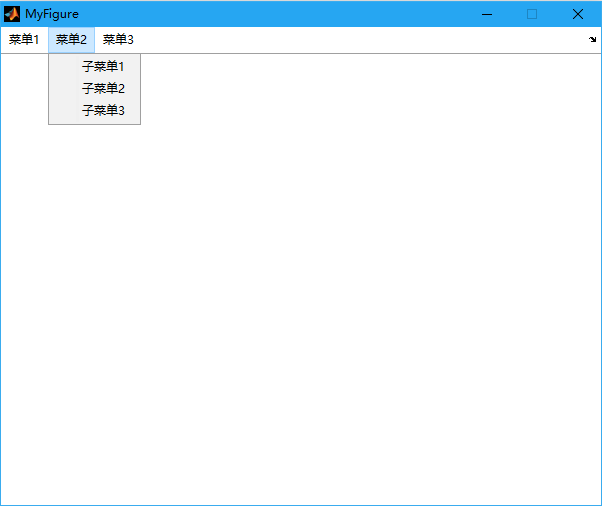
\includegraphics[scale=0.35]{MyFigure_uimenu}
		\caption{\textbf{带菜单的MyFigure窗口}}
	\end{figure}
	继续添加如下代码运行测试,运行结果为图2-5。
	\begin{lstlisting}
 ui = 1:4;												% 创建控件数组
 string = {'text','edit','pushbutton','popup'};			% 创建控件名称字符串数组
 position = [100,380,240,25								% 创建位置和大小的二级数组
             100,350,240,25
 			 100,320,240,25
             100,290,240,25];
 for i = 1:length(ui)									% 利用 for 循环创建控件和设置属性参数
     ui(i) = uicontrol(hf,...							% 设置父对象
         'Style',string{i},...							% 设置控件类型,调用 string 数组
         'FontSize',10,...								% 设置字体大小
		 'Tag',string{i},...							% 设置 Tag 标签
         'Units','pixels',...							% 设置位置大小设置类型为像素
         'String',string{i},...							% 设置显示的字符串
         'Position',position(i,:));						% 设置位置和大小,调用二维数组
 end\end{lstlisting}
 	\begin{figure}[H]
		\centering
		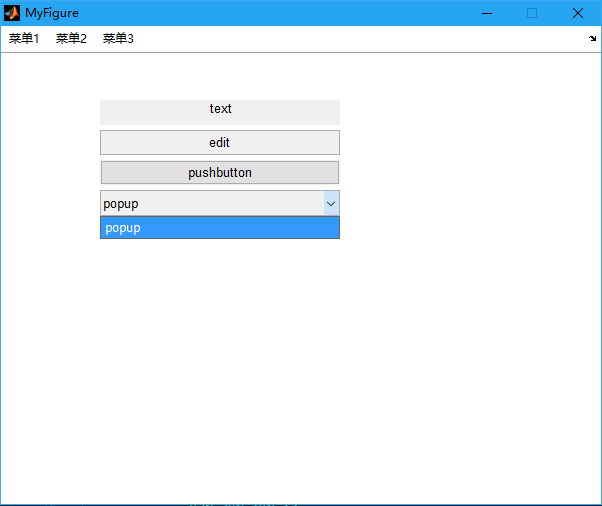
\includegraphics[scale=0.35]{MyFigure_uicontrol}
		\caption{\textbf{带控件的MyFigure窗口}}
	\end{figure}
	以后界面中的控件设计就用此函数实现,利用for循环和定义属性值数组可以更灵活的创建控件和设置控件的属性。该毕业设计的界面控件设计就是利用此方法来实现控件的布局和大小设置。
	\item \textbf{uipanel函数}

	\qquad uipanel函数可以创建一个面板来归类控件,使界面的控件更直观,实现的函数如下:
	\begin{lstlisting}
 ui = uipanel(parent,'PropertyName',propertyvalue,...);\end{lstlisting}
 	其中的参数属性设置和前面的函数一样。继续向前面的m文件中追加如下代码,运行结果如图2-6。
	\begin{lstlisting}
 up = uipanel(hf,...									% 设置父对象
 	'Title','uipanel',...								% 设置名称
 	'FontSize',10,...									% 设置字体大小
 	'Units','pixels',...								% 设置位置大小设置类型为像素
 	'Position',[100,100,350,160]);						% 设置位置和大小\end{lstlisting}
	\begin{figure}[H]
		\centering
		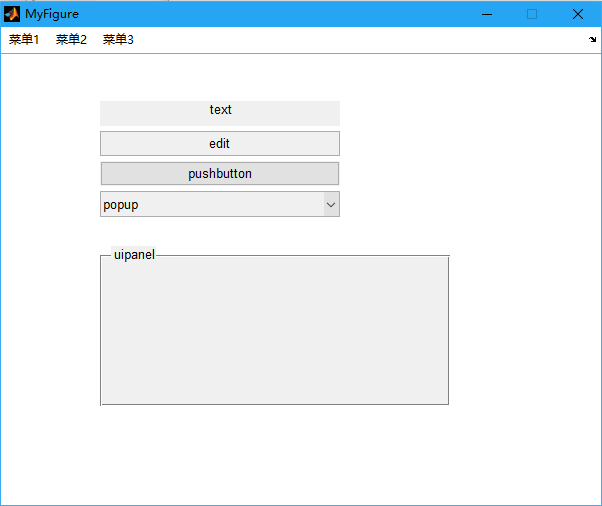
\includegraphics[scale=0.35]{MyFigure_uipanel}
		\caption{\textbf{带面板的MyFigure窗口}}
	\end{figure}
	\item \textbf{axes函数}

	\qquad 在界面设计的过程中,要想在界面上绘制函数图像,则必须创建axes坐标轴,创建方法如下:
	\begin{lstlisting}
 ua = axes('PropertyName',propertyvalue,...);\end{lstlisting}
 	其中的参数属性设置和前面的函数一样。继续向前面的m文件中追加如下代码,运行结果如图2-7。
	 \begin{lstlisting}
 ua = axes(...											% 定义坐标轴对象名为 ua
	'Units','pixels',...								% 设置位置大小设置类型为像素
	'Position',[100,100,350,160]);						% 设置位置和大小
	x = 0:0.01:2*pi;
	y = sin(x);
	axes(ua);											% 设置绘图的坐标轴为 ua
	plot(x,y);\end{lstlisting}
	\begin{figure}[H]
		\centering
		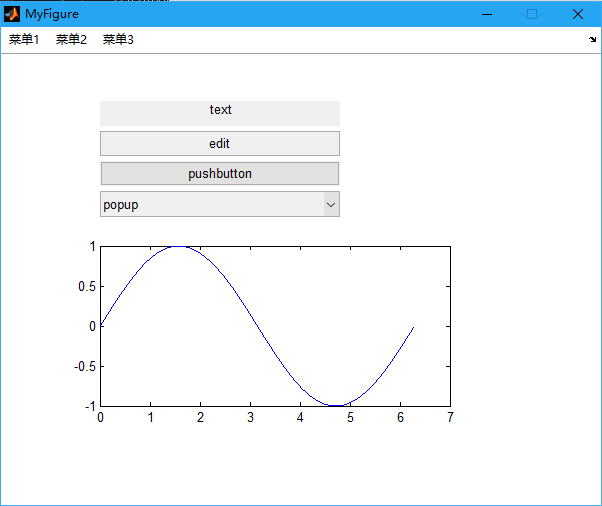
\includegraphics[scale=0.35]{MyFigure_axes}
		\caption{\textbf{带坐标轴的MyFigure窗口}}
	\end{figure}
\end{enumerate}

利用前面的5个GUI设计函数,可以设计出任何图形交互界面,只需要在函数参数中根据需求设置属性即可,控件中常用的属性设置见附录B,但上面的仅仅是设计好界面,还不能够处理数据,要想使用控件触发事件,则需要使用回调函数。
\subsubsection{Matlab中回调函数的编写}
GUI界面中,要想实现数据的交互和计算处理,要用到下面三个函数来获取界面控件属性的值和设置界面控件的属性。
\begin{enumerate}
	\item \textbf{get函数}

	\qquad 使用get函数可以获取对象的属性值,get函数的形式如下:
	\begin{lstlisting}
 get(h,'PropertyName');\end{lstlisting}
 	其中:h为要获取的对象,可以是控件、菜单、窗口等,PropertyName为要获取属性值的属性名称。在前面的代码中添加下面代码:
	 \begin{lstlisting}
 get(ui(3),'String')									% 获取 ui(3) 控件的 String 属性\end{lstlisting}
 	因为上面代码没有写分号,运行结果会在命令窗口输出pushbutton,因为ui(3)是之前创建的按钮控件。
	\item \textbf{set函数}

	\qquad 使用set函数可以设置对象的属性值,set函数的形式如下:
	\begin{lstlisting}
 set(h,'PropertyName',propertyvalue,...);\end{lstlisting}
 	其中:h为要设置的对象,可以是控件、菜单、窗口等,PropertyName为要设置属性的名称,propertyvalue为要设置的属性值。在前面的代码中添加下面代码:
	 \begin{lstlisting}
 set(ui(1),'String',1);									% 设置 ui(1) 控件的 String 属性为1\end{lstlisting}
 	运行结果可以发现界面中text已经变成1了,因为创建的ui(1)为静态文本控件。
	\item \textbf{guidata函数}

	\qquad 这个函数可以用来存储和获取GUI界面的控件数据,每个控件在Matlab中都有一个ID,主界面的所有控件ID都存放在一个数组里,guidata函数可以将ID以结构体的形式保存起来,结构体中有控件的Tag属性和ID,然后可以在回调函数中利用guidata函数来获取需要设置的控件。将前面的代码改成m函数文件,再添加如下代码:
	\begin{lstlisting}
 function MyFrame										% 创建 m 函数文件,名称与文件名称一致
 hf = figure('Name','MyFigure',...						% 省略前面写好的代码
 ......
 set(ui(3),'Callback',@fun_plot);						% 设置按钮的回调函数为fun_plot
 guidata(hf,guihandles);								% 将控件 guihandles 保存在窗口对象变量 hf 中

 function fun_plot(cbo,handles)							% 创建回调函数
 handles = guidata(cbo)									% 根据按钮来获取前面保存的数据
 set(handles.text,'String',2);							% 设置 text 的 String 属性为2\end{lstlisting}
 	运行上面的函数文件,然后单击按钮,就会在命令窗口打印下面的信息,它是所有带Tag属性控件的结构体,信息包含控件Tag和ID,单击按钮后还会使text的String属性变成2。设置和获取属性时用handles.Tag来获取控件。
	\begin{lstlisting}
 handles = 
         popup: 9.0455
    pushbutton: 8.0455
          edit: 7.0455
          text: 6.0455\end{lstlisting}
\end{enumerate}

通过设置回调函数,设置界面控件数据的保存和读取,可以完成界面处理数据的功能。编写界面的代码以及回调子函数都可以放在一个m函数文中。在需要添加事件的控件增加Callback属性,属性值为@加子函数名,当控件被触发,会执行Callback设置的子函数,比如:按钮的单击、下拉列表的选择、滚动条的选值等,都可以触发Callback。还有一些别的回调函数,比如CreateFcn属性,它是设置对象创建时执行的回调函数,更多回调函数属性见附录B。

\subsection{误差理论与数据处理GUI界面设计}
在基于GUI的误差理论与数据处理系统设计中,整个软件项目分为两个部分,一部分是界面和控件回调函数的代码,另一部分是误差数据处理部分。按实现的功能分,共有三级界面,总界面:有学校名称(中英文)、学校校徽、校训、代表性建筑,《误差理论与数据处理》中英文名称。二级界面,点击总界面中《误差理论与数据处理》进入二级界面,二级界面包括:测量数据基本处理、误差的合成、测量不确定度、最小二乘法处理、回归分析五个部分。三级界面,测量数据基本处理中三级界面包括:等精度测量数据误差分析、不等精度测量数据误差分析,最小二乘法处理中三级界面包括:等精度测量线性参数最小二乘法处理、不等精度测量线性参数最小二乘法处理,误差的合成即为三级界面,测量不确定度,即为三级界面,回归分析,即为三级界面。比如主界面的设计分为三个部分:界面和控件的设计、回调函数的编写、界面的优化。
\newpage
\begin{enumerate}
	\item	\textbf{界面和控件的设计}
	
	\qquad 首先,创建一个m函数文件index.m,主函数名与文件名一致,然后用figure函数创建一个界面,并设置相应的属性,代码如下:
	\begin{lstlisting}
 function index										% 主函数
		
 %% 创建主界面
 hf = figure('Name','基于GUI的误差理论与数据处理系统',...	% 界面的名称
 	'NumberTitle','off',...							% 取消显示界面名称编号
 	'Units','pixels',...							% 设置长度单位为像素
 	'Position',[200,200,600,450],...				% 设置界面的位置与大小
 	'MenuBar','none',...							% 取消默认菜单
 	'Color','White',...								% 背景颜色为白色
 	'Resize','off');								% 禁止改变界面大小\end{lstlisting}
 	\qquad 然后,在前面创建好界面的基础上,使用uicontrol创建控件,界面中只要显示文字和图片。显示文字用静态文本,添加以下代码创建静态文本控件:
 	\begin{lstlisting}
 % 校训
 uicontrol(hf,...									% 第一个属性为父类对象名
 	'Units','pixels',...							% 设置长度单位为像素
 	'Position',[300,320,230,25],...					% 设置控件的位置和大小
 	'Style','text',...								% 控件的类型为文本
 	'String','崇德博智,扶危定倾',...				% 设置显示的字符串
 	'FontName','楷体',...							  % 字体
 	'FontSize',18,...								% 字号
 	'FontWeight','bold',...							% 字体加粗
 	'ForegroundColor',[7,51,123]/255,...			% 设置颜色,值为 RGB 色彩
 	'BackgroundColor','White');						% 背景颜色
 %% 《误差理论与数据处理》中文名称
 uicontrol(hf,...									% 第一个属性为父类对象名
 	'Units','pixels',...							% 设置长度单位为像素
 	'Position',[160,35,280,25],...					% 设置界面的位置和大小
 	'Style','text',...								% 控件的类型为文本
 	'String','《误差理论与数据处理》',...			  % 设置显示的字符串
 	'FontName','楷体',...							  % 字体
 	'FontSize',18,...								% 字号
 	'FontWeight','bold',...							% 字体加粗
 	'ForegroundColor',[7,51,123]/255,...			% 设置颜色,值为 RGB 色彩
 	'BackgroundColor','White');						% 背景颜色
 %% 《误差理论与数据处理》英文名称
 uicontrol(hf,...									% 第一个属性为父类对象名
 	'Units','pixels',...							% 设置长度单位为像素
 	'Position',[160,5,280,25],...					% 设置控件的位置和大小
 	'Style','text',...								% 控件的类型为文本
 	'String','Error Theory and Data Processing',...	% 设置显示的字符串.
 	'FontSize',12,...								% 字号
 	'FontWeight','bold',...							% 字体加粗
 	'ForegroundColor',[7,51,123]/255,...			% 设置颜色,值为 RGB 色彩
 	'BackgroundColor','White');						% 背景颜色\end{lstlisting}
 	\qquad 创建好静态文本后,在界面中放置图片,在Matlab不能直接地放置图片,所以需要在主窗口上添加一个axes控件,该控件的位置和大小设置成图片的位置和大小,在控件的属性CreateFcn的函数下添加嵌入图片的代码\scite{3},例如:X=imread(’图片文件名’),imshow(X)。所以用axes函数添加坐标轴,代码如下:
 	\begin{lstlisting}
 % 学校图标和名称
 axes('Units','pixels',...							% 设置长度单位为像素
 	'Position',[0,350,430,100]);					% 设置 axes 的位置和大小
 % 学校标志性建筑
 axes('Units','pixels',...							% 设置长度单位为像素
 	'Position',[0,80,600,233]);						% 设置 axes 的位置和大小\end{lstlisting}
 	\item	\textbf{回调函数的编写}
 	
 	\qquad 界面已经设计好,所有控件的位置和大小都已调整好,此时,文字按钮还不能在单击后进入二级界面,图片也没有显示,这些都要编写回调函数来完成。在《误差理论与数据处理》中文名称和英文名称的静态文本控件中都添加下面属性:
 	\begin{lstlisting}
 'enable','inactive',...							% 禁止执行回调字符串
 'ButtonDownFcn','subpage',...						% 设置单击回调函数\end{lstlisting}
 	\qquad 上面代码中,subpage为子界面的m文件,单击此控件就会打开子界面。在用来显示学校图标和名称图片的axes函数中添加下面属性:
 	\begin{lstlisting}
 'CreateFcn',@school_logo,...						% 设置控件创建时的回调函数\end{lstlisting}
 	\qquad 然后在当前m函数文件后面添加回调子函数用来执行显示图片的代码。
 	\begin{lstlisting}
 % 显示学校名称PNG图片函数
 function school_logo(cbo,handles)					% 创建子函数
 [I,c,alpha] = imread('image/school_logo.png');		% 读取图片数据
 h = imshow(I);										% 显示图片
 set(h,'AlphaData',alpha);							% 设置透明度\end{lstlisting}
 	\qquad 此时,学校图标和名称已经显示出来了,注意imread函数的参数为图片的路径和文件名。再继续在显示学校标志性建筑的axes中添加下面属性:
 	\begin{lstlisting}
 'CreateFcn','imshow(''image/school.jpg'')',...		% 设置显示的图片\end{lstlisting}
 \begin{figure}[H]
 	\centering
 	
\includegraphics[scale=0.4]{index}
 	\caption{\textbf{主界面}}
 \end{figure}
 	\qquad 在回调函数中,可以把执行的语句直接写在属性值里面,也可以用@来调用子函数。到这已经实现了图片的显示和界面的跳转,写好子界面subpage.m的话,就可以单击上面的控件跳转到子界面了,整个主界面运行的结果如图2-8。
 	\item	\textbf{界面的优化}
 	
 	\qquad 界面编写好后对其优化,使它执行起来更稳定,增强它的兼容性。首先,在文件中主函数前面添加clear和clc,用来清除执行前的Matlab数据,再使用addpath函数添加项目文件的路径,因为以后的项目文件都必须加入Matlab的环境路径中才能执行该目录下的所有m文件。
 	\begin{lstlisting}
 function index
 clear												% 清除数据
 clc												% 清除命令窗口
 addpath(genpath(pwd));								% 添加子文件夹路径
 %% 创建主界面
 s = get(0,'ScreenSize');							% 获取计算机屏幕分辨率
 x = s(3)*0.15;										% 设置界面的 x 坐标为屏幕的15%
 y = s(4)*0.26;										% 设置界面的 y 坐标为屏幕的26%
 hf = figure('Name','基于...系统',...
 	...
 	'Position',[x,y,600,450],...					% 将位置改为 x 和 y
 	...);\end{lstlisting}
 	\qquad 然后使用get函数来获取计算机屏幕的分辨率,根据分辨率来设置主界面的位置,这样就可以适应不同分辨率的计算机。更改界面左上角的图标,图形界面默认的图标是Matlab软件图标,在主函数中添加下面代码,如图2-8,左上角图标已经换成学校logo。
 	\begin{lstlisting}
 % 更改界面左上角图标
 newIcon = javax.swing.ImageIcon('./image/logo.png');
 figFrame = get(gcf,'JavaFrame');
 figFrame.setFigureIcon(newIcon);\end{lstlisting}
 	\qquad 添加退出确认对话框,在主界面创建函数中添加CloseRequestFcn属性,然后再编写子函数执行对话框,代码如下:
 	\begin{lstlisting}
 'CloseRequestFcn',@hexit,...						% 添加至 figure 函数中的属性
 
 %% 主界面退出对话框
 function hexit(cbo,handles)						% 退出执行的回调函数
 he = questdlg('你确定退出吗?','退出程序','是','否','否');	% 提问对话框函数
 if strcmp(he,'是')								   % 判断对话框按钮的动作
	 close;
	 clear;
	 clc;
 end;\end{lstlisting}
 	\qquad 整个代码文件见附录C,主界面的全部功能已经编写完成,其它子界面,其原理都是一样的,项目源代码见附件或者 \url{https://github.com/AiJiangnan/ErrorTheoryDataProcessing}。
\end{enumerate}